\documentclass{standalone}
\usepackage{tikz}
\usetikzlibrary{patterns}
\usetikzlibrary{positioning}
\usetikzlibrary{patterns, positioning}
\usetikzlibrary{shapes.misc}
\usepackage[outline]{contour}
\contourlength{1.5pt} 
\usepackage[sfdefault]{ClearSans}

\begin{document}
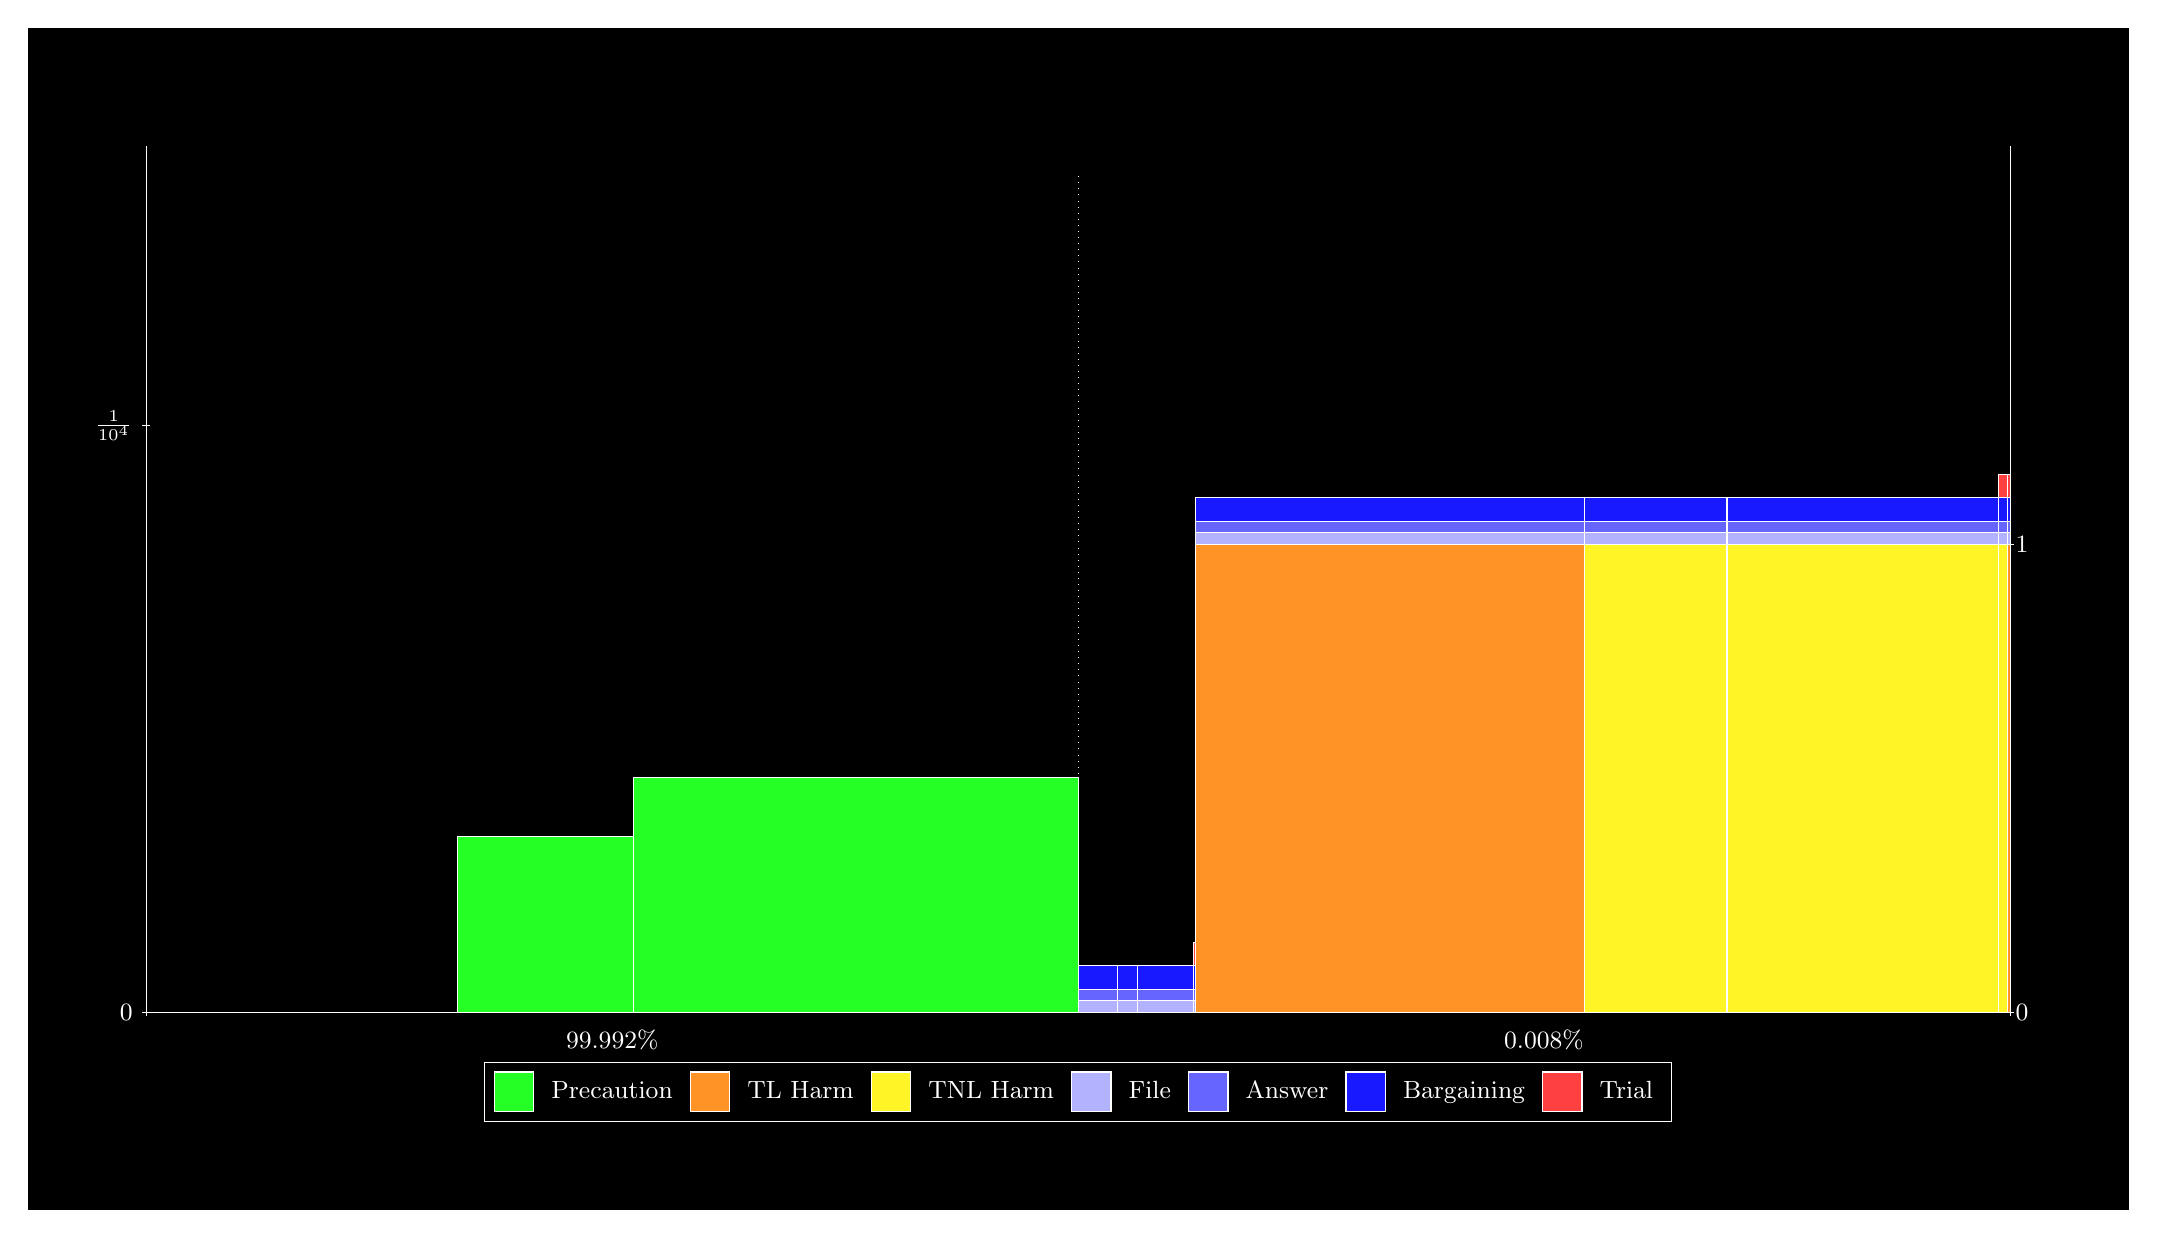
\begin{tikzpicture}
\draw[fill=black] (0,0) rectangle (26.667,15);
\draw[fill=green!85,draw=white,very thin] (5.4443,2.5) rectangle (7.6851,4.7362);
\draw[fill=green!85,draw=white,very thin] (7.6851,2.5) rectangle (13.333,5.4816);
\draw[fill=blue!30,draw=white,very thin] (13.333,2.5) rectangle (13.828,2.6486);
\draw[fill=blue!60,draw=white,very thin] (13.333,2.6486) rectangle (13.828,2.7972);
\draw[fill=blue!90,draw=white,very thin] (13.333,2.7972) rectangle (13.828,3.0944);
\draw[fill=green!85,draw=white,very thin] (13.828,2.5) rectangle (14.084,2.5002);
\draw[fill=blue!30,draw=white,very thin] (13.828,2.5002) rectangle (14.084,2.6488);
\draw[fill=blue!60,draw=white,very thin] (13.828,2.6488) rectangle (14.084,2.7974);
\draw[fill=blue!90,draw=white,very thin] (13.828,2.7974) rectangle (14.084,3.0945);
\draw[fill=green!85,draw=white,very thin] (14.084,2.5) rectangle (14.792,2.5002);
\draw[fill=blue!30,draw=white,very thin] (14.084,2.5002) rectangle (14.792,2.6488);
\draw[fill=blue!60,draw=white,very thin] (14.084,2.6488) rectangle (14.792,2.7974);
\draw[fill=blue!90,draw=white,very thin] (14.084,2.7974) rectangle (14.792,3.0946);
\draw[fill=green!85,draw=white,very thin] (14.792,2.5) rectangle (14.817,2.5002);
\draw[fill=blue!30,draw=white,very thin] (14.792,2.5002) rectangle (14.817,2.6488);
\draw[fill=blue!60,draw=white,very thin] (14.792,2.6488) rectangle (14.817,2.7974);
\draw[fill=blue!90,draw=white,very thin] (14.792,2.7974) rectangle (14.817,3.0945);
\draw[fill=red!75,draw=white,very thin] (14.792,3.0945) rectangle (14.817,3.3917);
\draw[fill=orange!85,draw=white,very thin] (14.817,2.5) rectangle (19.764,8.4436);
\draw[fill=blue!30,draw=white,very thin] (14.817,8.4436) rectangle (19.764,8.5922);
\draw[fill=blue!60,draw=white,very thin] (14.817,8.5922) rectangle (19.764,8.7408);
\draw[fill=blue!90,draw=white,very thin] (14.817,8.7408) rectangle (19.764,9.038);
\draw[fill=green!85,draw=white,very thin] (19.764,2.5) rectangle (21.566,2.5002);
\draw[fill=yellow!85,draw=white,very thin] (19.764,2.5002) rectangle (21.566,8.4438);
\draw[fill=blue!30,draw=white,very thin] (19.764,8.4438) rectangle (21.566,8.5924);
\draw[fill=blue!60,draw=white,very thin] (19.764,8.5924) rectangle (21.566,8.741);
\draw[fill=blue!90,draw=white,very thin] (19.764,8.741) rectangle (21.566,9.0381);
\draw[fill=green!85,draw=white,very thin] (21.566,2.5) rectangle (21.58,2.5002);
\draw[fill=orange!85,draw=white,very thin] (21.566,2.5002) rectangle (21.58,8.4438);
\draw[fill=blue!30,draw=white,very thin] (21.566,8.4438) rectangle (21.58,8.5924);
\draw[fill=blue!60,draw=white,very thin] (21.566,8.5924) rectangle (21.58,8.741);
\draw[fill=blue!90,draw=white,very thin] (21.566,8.741) rectangle (21.58,9.0381);
\draw[fill=green!85,draw=white,very thin] (21.58,2.5) rectangle (25.015,2.5002);
\draw[fill=yellow!85,draw=white,very thin] (21.58,2.5002) rectangle (25.015,8.4438);
\draw[fill=blue!30,draw=white,very thin] (21.58,8.4438) rectangle (25.015,8.5924);
\draw[fill=blue!60,draw=white,very thin] (21.58,8.5924) rectangle (25.015,8.741);
\draw[fill=blue!90,draw=white,very thin] (21.58,8.741) rectangle (25.015,9.0382);
\draw[fill=green!85,draw=white,very thin] (25.015,2.5) rectangle (25.132,2.5002);
\draw[fill=yellow!85,draw=white,very thin] (25.015,2.5002) rectangle (25.132,8.4438);
\draw[fill=blue!30,draw=white,very thin] (25.015,8.4438) rectangle (25.132,8.5924);
\draw[fill=blue!60,draw=white,very thin] (25.015,8.5924) rectangle (25.132,8.741);
\draw[fill=blue!90,draw=white,very thin] (25.015,8.741) rectangle (25.132,9.0381);
\draw[fill=red!75,draw=white,very thin] (25.015,9.0381) rectangle (25.132,9.3353);
\draw[fill=green!85,draw=white,very thin] (25.132,2.5) rectangle (25.167,2.5002);
\draw[fill=orange!85,draw=white,very thin] (25.132,2.5002) rectangle (25.167,8.4438);
\draw[fill=blue!30,draw=white,very thin] (25.132,8.4438) rectangle (25.167,8.5924);
\draw[fill=blue!60,draw=white,very thin] (25.132,8.5924) rectangle (25.167,8.741);
\draw[fill=blue!90,draw=white,very thin] (25.132,8.741) rectangle (25.167,9.0381);
\draw[fill=red!75,draw=white,very thin] (25.132,9.0381) rectangle (25.167,9.3353);
\draw[white,very thin] (1.5,2.5) -- (1.5,13.5);
\draw[white,very thin] (1.45,2.5) -- (1.55,2.5);
\node[font=\small,text=white, anchor=east] at (1.45, 2.5) {0};
\draw[white,very thin] (1.45,9.9539) -- (1.55,9.9539);
\node[font=\small,text=white, anchor=east] at (1.45, 9.9539) {$\frac{1}{10^{4}}$};

\draw[white,dotted,very thin] (13.333,2.83) -- (13.333,13.17);
\draw[white,very thin] (25.167,2.5) -- (25.167,13.5);
\draw[white,very thin] (25.117,2.5) -- (25.217,2.5);
\node[font=\small,text=white, anchor=west] at (25.117, 2.5) {0};
\draw[white,very thin] (25.117,8.4436) -- (25.217,8.4436);
\node[font=\small,text=white, anchor=west] at (25.117, 8.4436) {1};

\draw[white,very thin] (1.5,2.5) -- (25.167,2.5);
\draw[white,very thin] (1.5,2.45) -- (1.5,2.55);
\node[font=\small,text=white, anchor=north] at (1.5, 2.45) {};
\draw[white,very thin] (25.167,2.45) -- (25.167,2.55);
\node[font=\small,text=white, anchor=north] at (25.167, 2.45) {};

\node[font=\small,text=white,anchor=south] at (7.4167, 1.9) {99.992\%};
\node[font=\small,text=white,anchor=south] at (19.25, 1.9) {0.008\%};
\draw (13.3333,2.5) node (B) {};
\begin{scope}[align=center]
\matrix[scale=0.5,draw=white,below=0.5cm of B,nodes={draw},column sep=0.1cm]{
\node[rectangle,draw,minimum width=0.5cm,minimum height=0.5cm,fill=green!85]{}; & \node[draw=none,font=\small,text=white]{Precaution}; &
\node[rectangle,draw,minimum width=0.5cm,minimum height=0.5cm,fill=orange!85]{}; & \node[draw=none,font=\small,text=white]{TL Harm}; &
\node[rectangle,draw,minimum width=0.5cm,minimum height=0.5cm,fill=yellow!85]{}; & \node[draw=none,font=\small,text=white]{TNL Harm}; &
\node[rectangle,draw,minimum width=0.5cm,minimum height=0.5cm,fill=blue!30]{}; & \node[draw=none,font=\small,text=white]{File}; &
\node[rectangle,draw,minimum width=0.5cm,minimum height=0.5cm,fill=blue!60]{}; & \node[draw=none,font=\small,text=white]{Answer}; &
\node[rectangle,draw,minimum width=0.5cm,minimum height=0.5cm,fill=blue!90]{}; & \node[draw=none,font=\small,text=white]{Bargaining}; &
\node[rectangle,draw,minimum width=0.5cm,minimum height=0.5cm,fill=red!75]{}; & \node[draw=none,font=\small,text=white]{Trial}; \\\\
};\end{scope}

\end{tikzpicture}
\end{document}